% Dieser Text ist urheberrechtlich gesch�tzt
% Er stellt einen Auszug eines von mir erstellten Referates dar
% und darf nicht gewerblich genutzt werden
% die private bzw. Studiums bezogen Nutzung ist frei
% Mai 2005 
% Autor: Sascha Frank 
% Universit�t Freiburg 
% www.informatik.uni-freiburg.de/~frank/


\documentclass{beamer}
\usepackage{color}
\definecolor{darkgreen}{rgb}{.008,.417,.067}
\usepackage{graphics}
\usepackage{pgf}
\beamertemplatenavigationsymbolsempty
 \usepackage{listings}
  \usepackage{courier}
 \lstset{
		 commentstyle=\tiny\ttfamily\color{darkgreen},
         basicstyle=\tiny\ttfamily, % Standardschrift
         %commentstyle=\fontsize{12}{14.4}\selectfont,
         %basicstyle=\ttfamily\fontsize{10}{12}\selectfont
         %numbers=left,               % Ort der Zeilennummern
         %numberstyle=\tiny,          % Stil der Zeilennummern
         %stepnumber=2,              % Abstand zwischen den Zeilennummern
         numbersep=3pt,              % Abstand der Nummern zum Text
         tabsize=2,                  % Groesse von Tabs
         extendedchars=true,         %
         breaklines=true,            % Zeilen werden Umgebrochen
         keywordstyle=\bfseries\ttfamily\color{orange},
         stringstyle=\color{green}\ttfamily,
         emph={rmc, gps_buffer_rmc},
         emphstyle=\color{blue}\texttt,
         %keywordstyle=\color{red}\textbf,
    	%	frame=b,         
         %keywordstyle=[1]\textbf,    % Stil der Keywords
         %keywordstyle=[2]\textbf,    %
         %keywordstyle=[3]\textbf,    %
         %keywordstyle=[4]\textbf,   %\sqrt{\sqrt{}} %
         %stringstyle=\color{white}\ttfamily, % Farbe der String
         showspaces=false,           % Leerzeichen anzeigen ?
         showtabs=false,             % Tabs anzeigen ?
         xleftmargin=17pt,
         framexleftmargin=17pt,
         framexrightmargin=5pt,
         framexbottommargin=4pt,
         %backgroundcolor=\color{lightgray},
         showstringspaces=false      % Leerzeichen in Strings anzeigen ?        
 }
 \lstloadlanguages{% Check Dokumentation for further languages ...
         %[Visual]Basic
         %Pascal
         C
         %C++
         %XML
         %HTML
         %Java
 }
%\DeclareCaptionFont{blue}{\color{blue}} 

%\captionsetup[lstlisting]{singlelinecheck=false, labelfont={blue}, textfont={blue}}
\usepackage{caption}
\DeclareCaptionFont{white}{\color{white}}
\DeclareCaptionFormat{listing}{\colorbox[cmyk]{0.43, 0.35, 0.35,0.01}{\parbox{\textwidth}{\hspace{15pt}#1#2#3}}}
\captionsetup[lstlisting]{format=listing,labelfont=white,textfont=white, singlelinecheck=false, margin=0pt, font={bf,footnotesize}}

\usetheme{Singapore}
\usefonttheme{professionalfonts}
\begin{document}
%\titlegraphic{\includegraphics[width=5cm,height=1cm]{Autosar_logo}}
\title{GPS Bycicle Computer}   
\author{Armin Schlegel\\Christian Eismann}
\date{\today} 

\begin{frame}
\titlepage
\end{frame} 

\section{Overview}
\subsection{Overview}
\begin{frame}
\frametitle{Overview}
\begin{itemize}
\item Introduction
\item The Toolchain
\item Hardware
\item Software
\item Conclusion
\end{itemize}
\end{frame}

\section{Introduction}
\subsection{Introduction}
\begin{frame}
\frametitle{The Project}
\textit{Development of a small device which provides multiple information on an on-board display that are
determined via the Global Positioning System}\\
Main components:
\begin{itemize}
\item GPS receiver
\item Graphic display
\item SD card (recording of GPS data)
\end{itemize}
\end{frame}

\begin{frame}
\frametitle{Tasks}
\begin{itemize}
\item definition of features
\item allocation of responsibilities
\item assembling of a toolchain
\item hardware development
\item software development
\item documentation
\end{itemize}
\end{frame}

\section{The Toolchain}
\subsection{The Toolchain}
\begin{frame}
\frametitle{Hardware/Software development tools}
Hardware:
\begin{itemize}
\item Eagle - circuit layout and design
\end{itemize}

Software:
\begin{itemize}
\item virtualbox (Oracle) including a Debian Linux image
\item GNU Compiler Collection (AVR-GCC)
\item avrdude (programmer)
\item Make
\item (sp)lint - static code analysis
\item ISP Programmer
\end{itemize}
\end{frame}

\begin{frame}
\frametitle{Software development tools}
Makefile warning options:\\
\lstinputlisting[language=make,label=gcc_compiler_warnings,caption=Compiler warnings]{Makefile_warnings.mak}
\end{frame}

\section{Hardware}
\subsection{Hardware}
\begin{frame}
\frametitle{Requirements}
Basic, rudimentary Requirements:
\begin{itemize}
\item Processor supply voltage: 3.3V
\item GPS receiver
\item RS232 Debug/Communication Port (choosable via jumper)
\item Usage of a graphic display
\item SD card for data recording
\item Mobile energy supply (chargeable)
\item programmable via ISP (and JTAG)
\end{itemize}
\end{frame}

\begin{frame}
\frametitle{Main components}
\begin{itemize}
\item ATmega32L and later ATmega644p (3.3V)
\item NL-552ETTL (GPS Receiver, 5V VCC, 3.3V RXD/TXD levels)
\item EA-DOGL128-6 (Display, 3.3V VCC, SPI)
\item YAMAICHI SD slot (3.3V VCC, SPI)
\item MAX3221 (RS232 controller, 3.3V VCC)
\end{itemize}
\end{frame}

\begin{frame}
\frametitle{Block diagram}
\begin{figure}
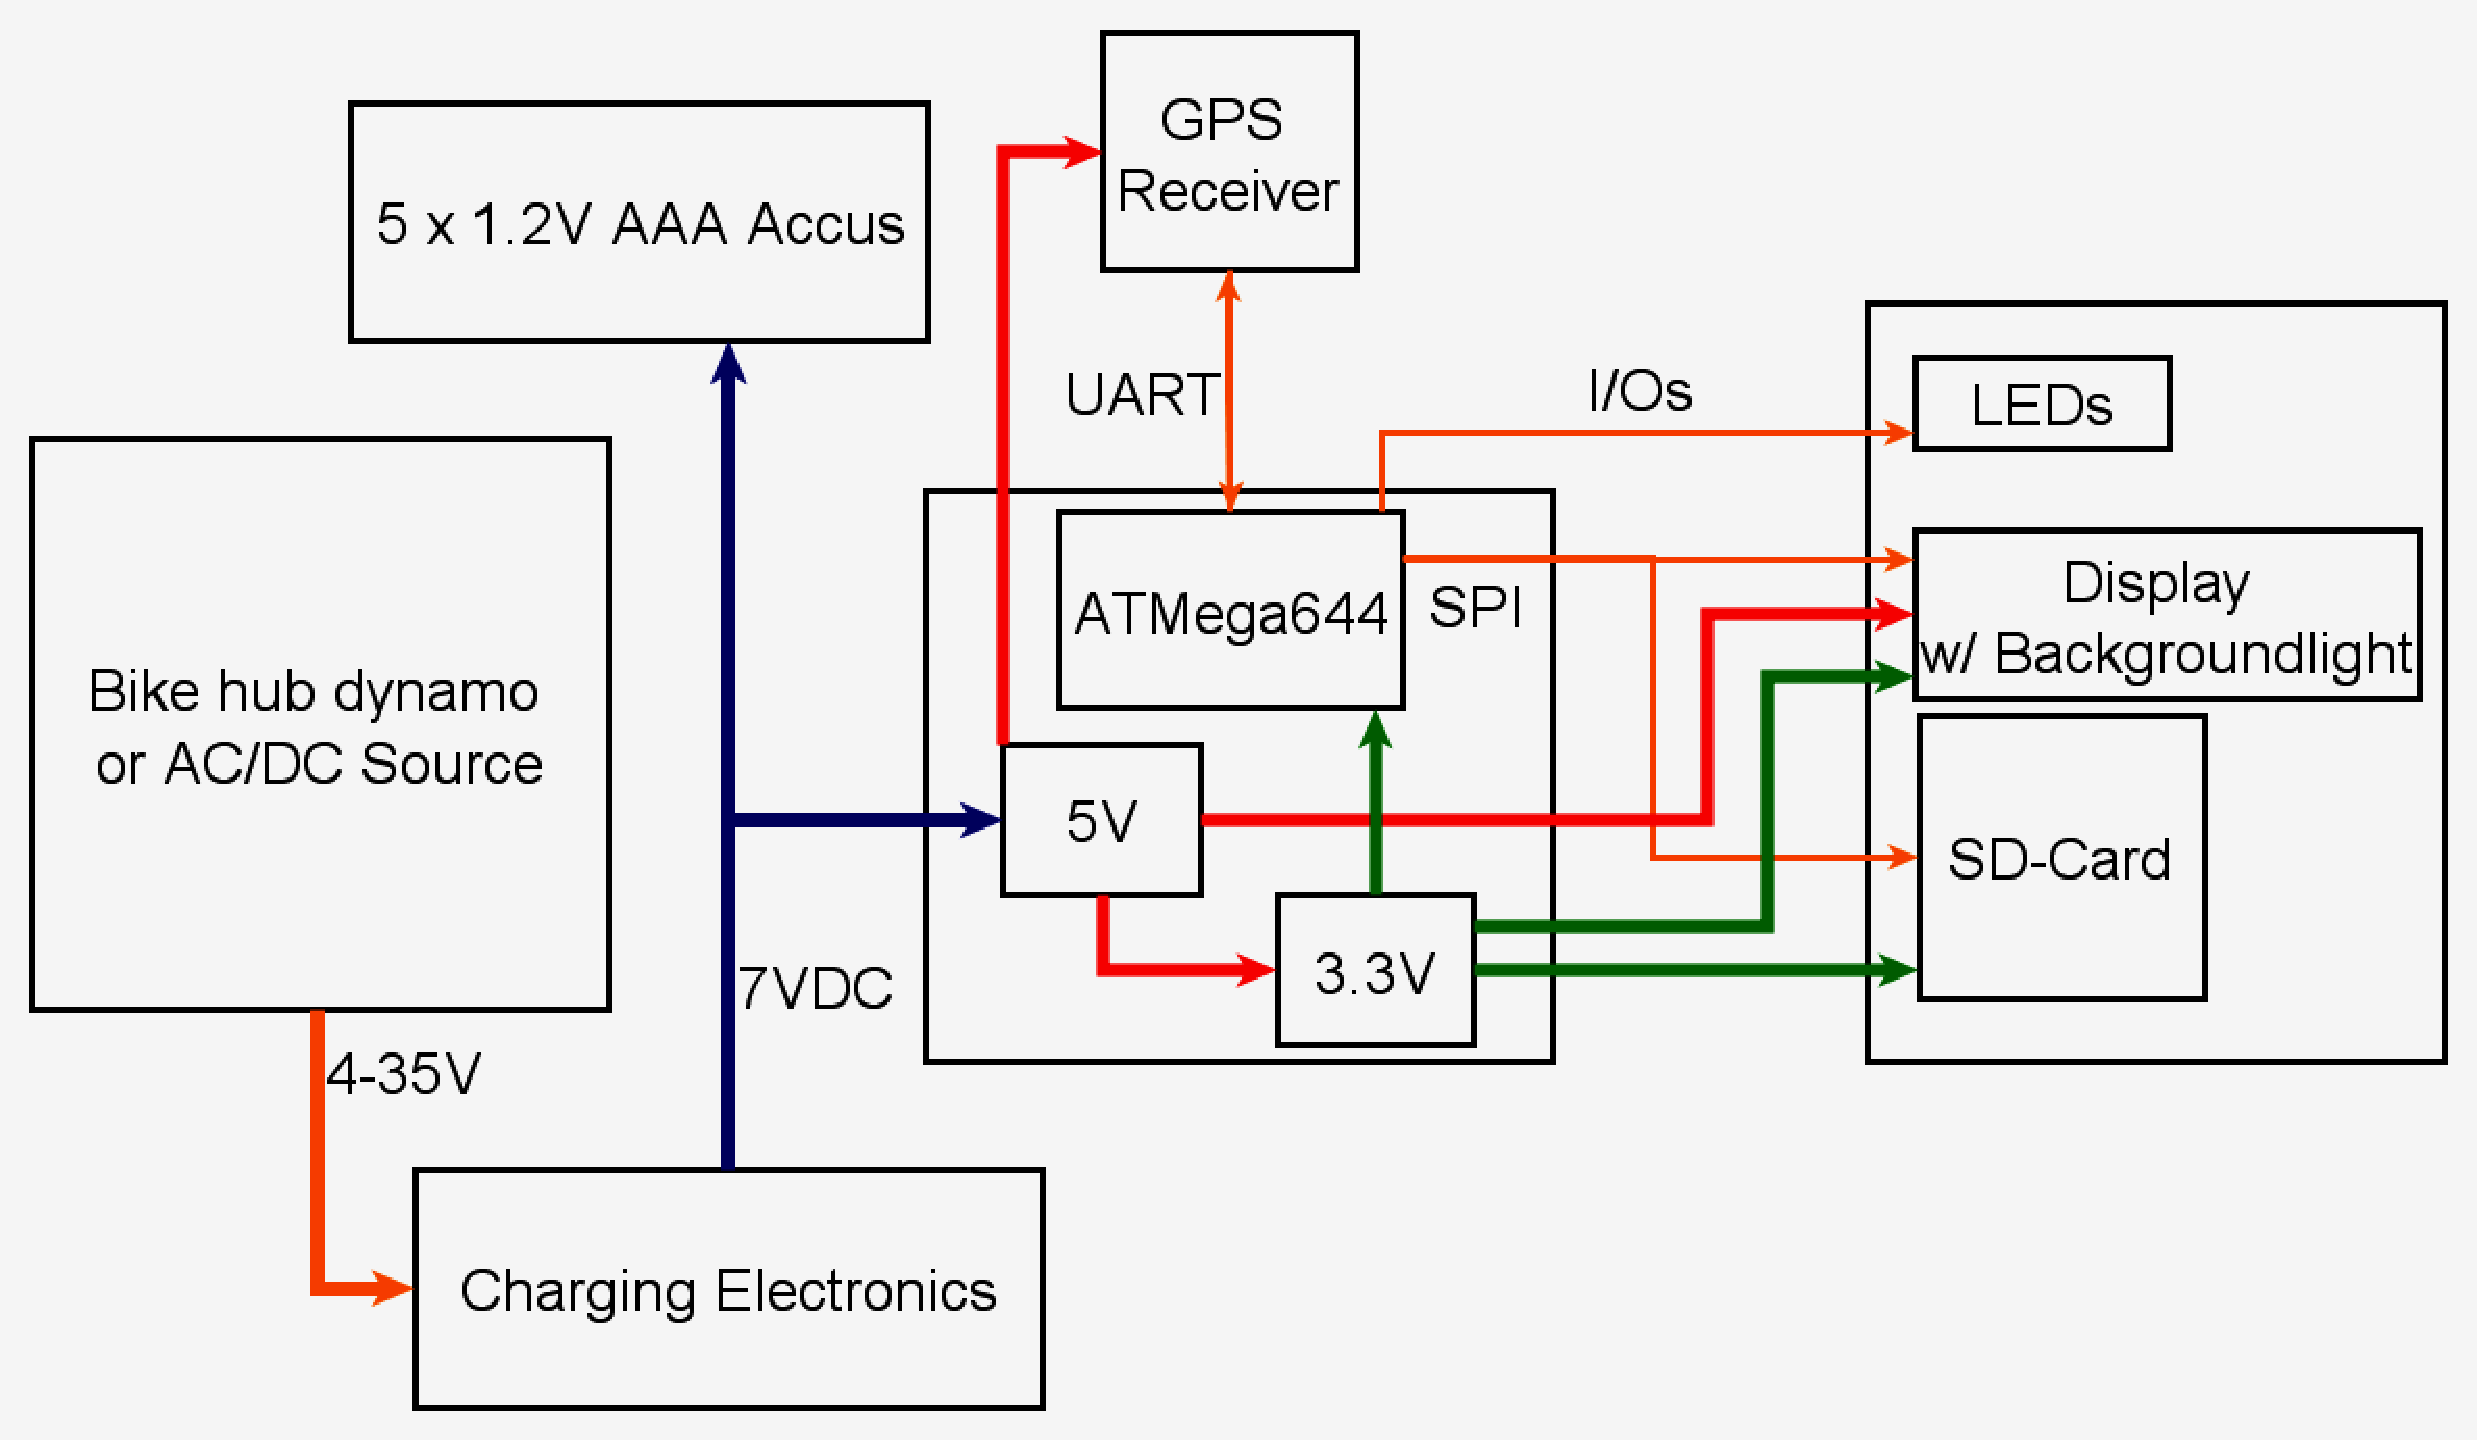
\includegraphics[width=\textwidth]{blockschaltbild}
\end{figure}
\end{frame}

\begin{frame}
\frametitle{Layout: main board}
\begin{figure}
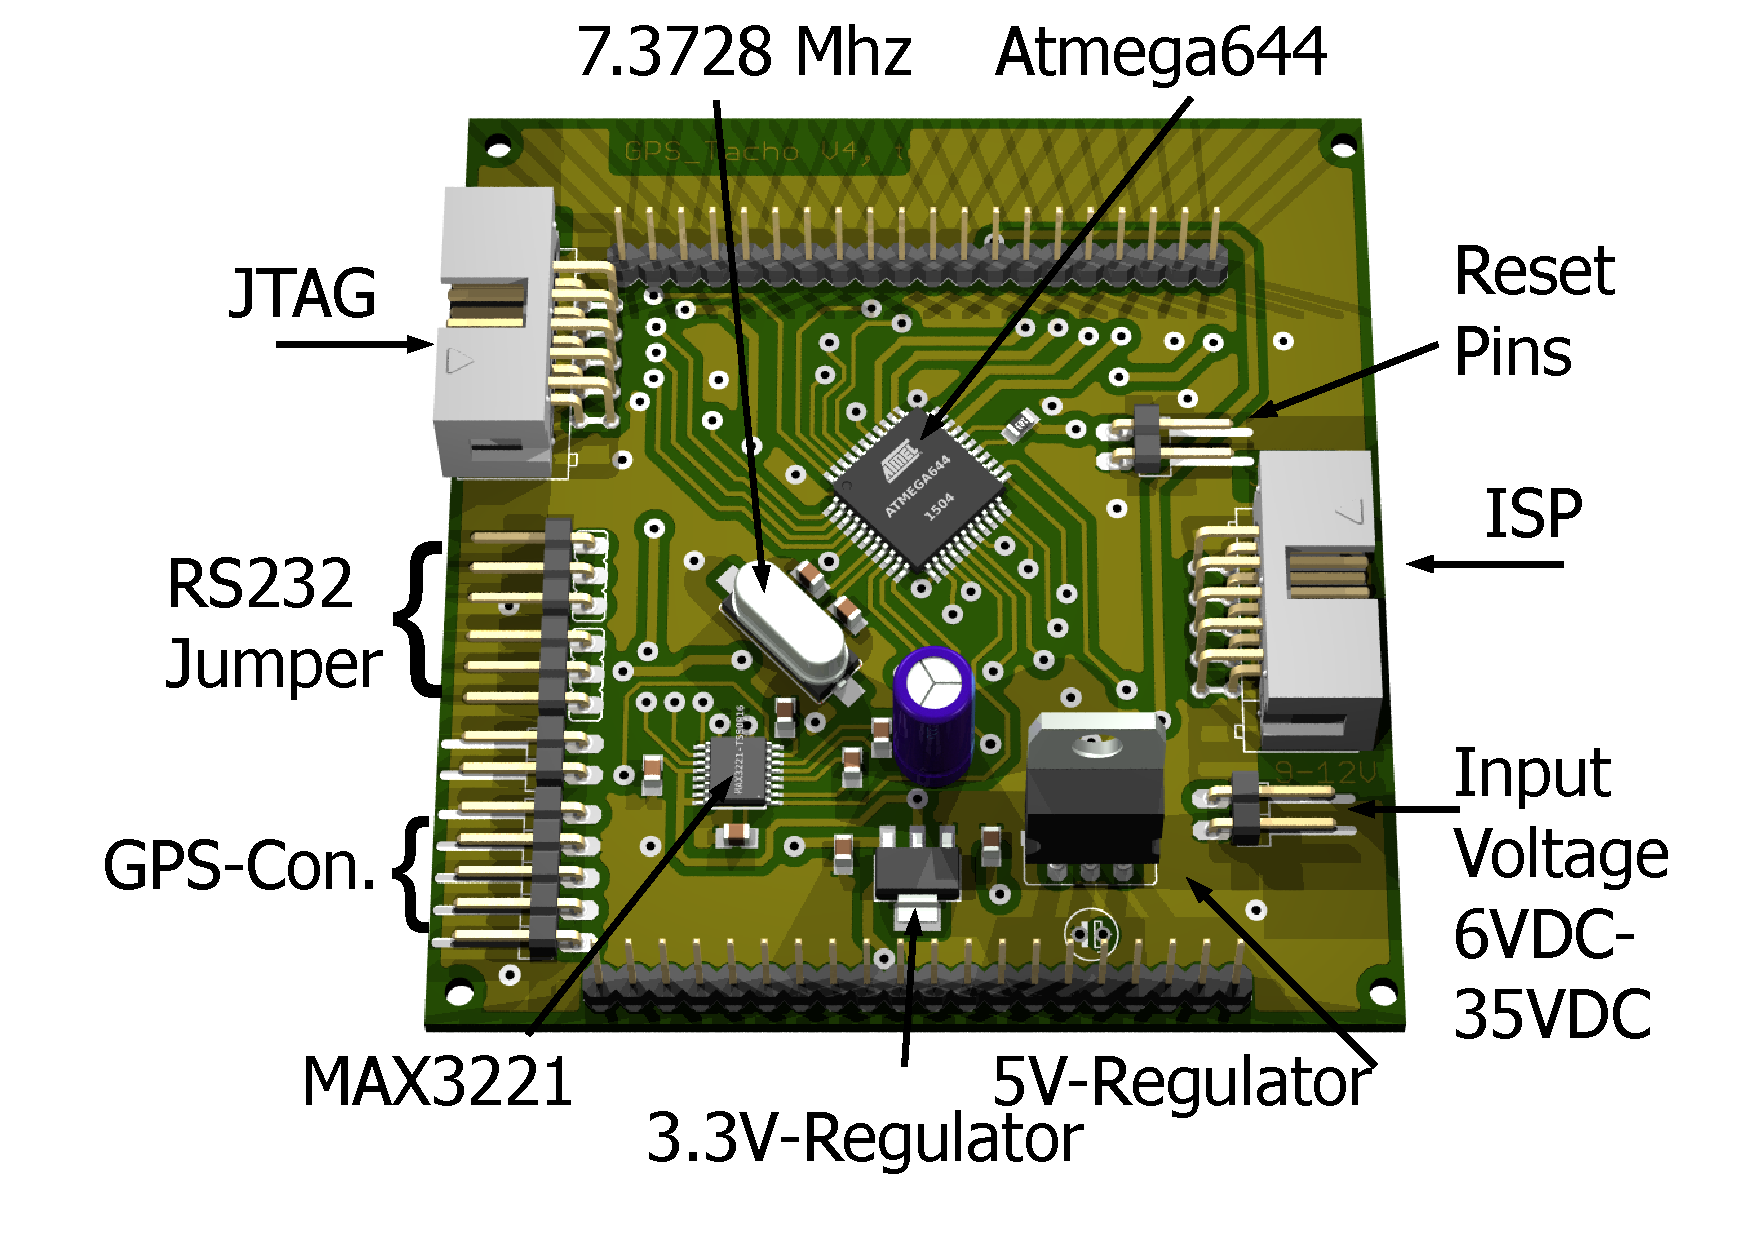
\includegraphics[width=\textwidth]{hardware_povray}
\end{figure}
\end{frame}

\begin{frame}
\frametitle{Comparison between oscillators}
\begin{figure}
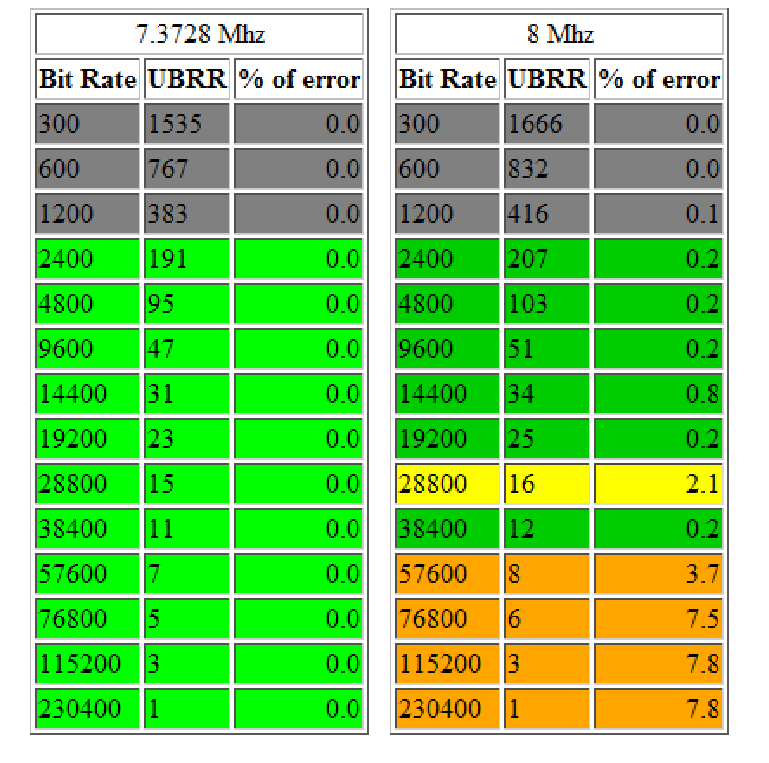
\includegraphics[width=0.7\textwidth]{osc_comp}
\end{figure}
\end{frame}

\section{Software}
\subsection{Software}
\begin{frame}
\frametitle{Design}
\begin{itemize}
\item mapping features to various modules
\item SW running synchronous to GPS data receiving (USART interrupt)
\item no usage of an OS
\end{itemize}
$\Rightarrow$ no timing/scheduling problems (general spoken: one big while(1) loop)
\end{frame}

\begin{frame}
\frametitle{The NMEA/PUBX Protocol}
\begin{figure}[htb]
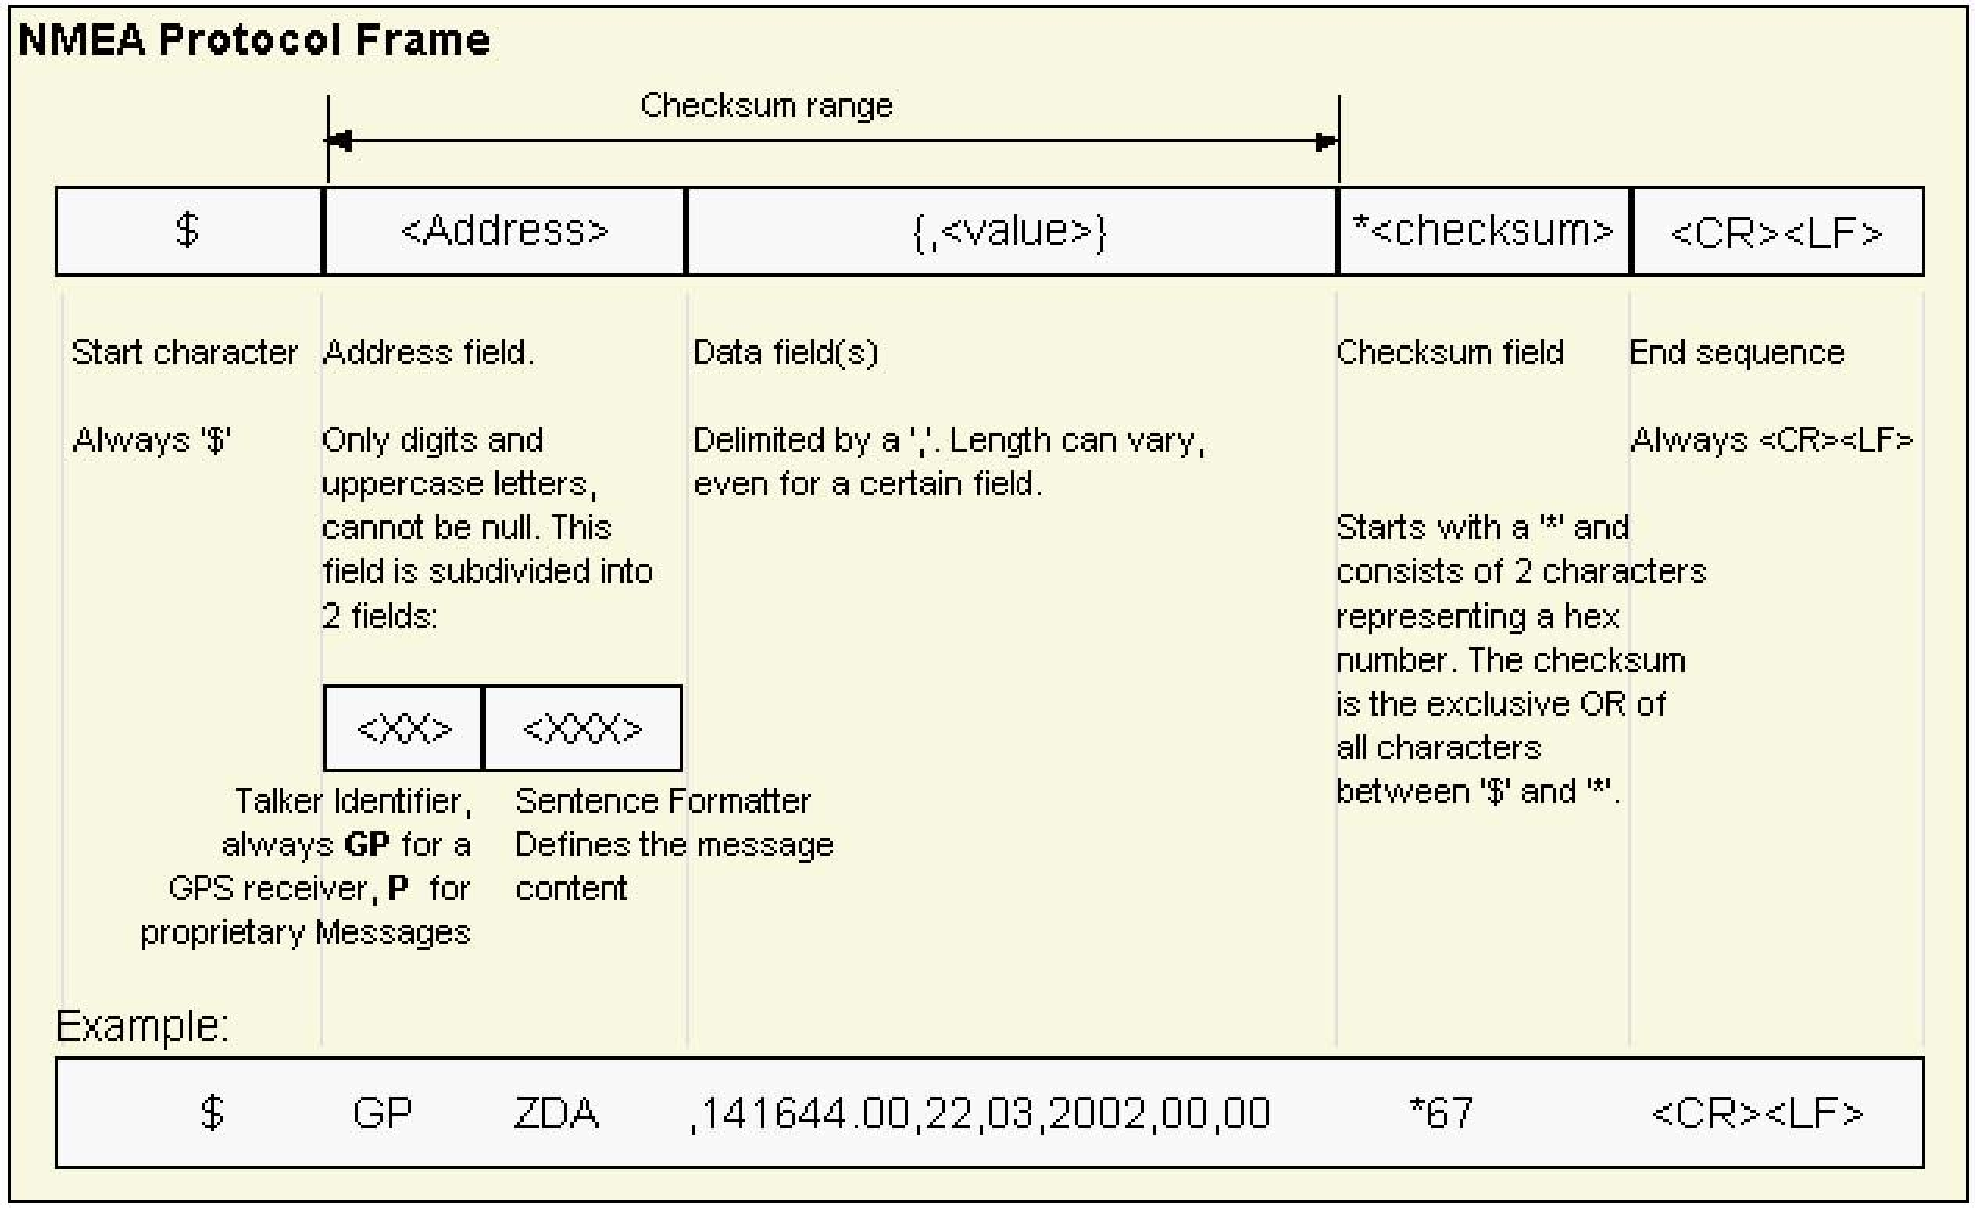
\includegraphics[width=\textwidth]{NMEA_protocol}
\end{figure}
\end{frame}

\begin{frame}
\frametitle{Components}
\begin{itemize}
\item SPI (Serial Peripheral Interface)
\begin{itemize}
\item Display
\item SDC/FAT16
\end{itemize}
\item UART (Universal Asynchronous Receiver Transmitter)
\begin{itemize}
\item GPS (Global Positioning System)
\end{itemize}
\item touch screen functionality via ADC
\item LEDs
\item application
\end{itemize}
\end{frame}

\begin{frame}
\frametitle{General workflow}
\begin{figure}
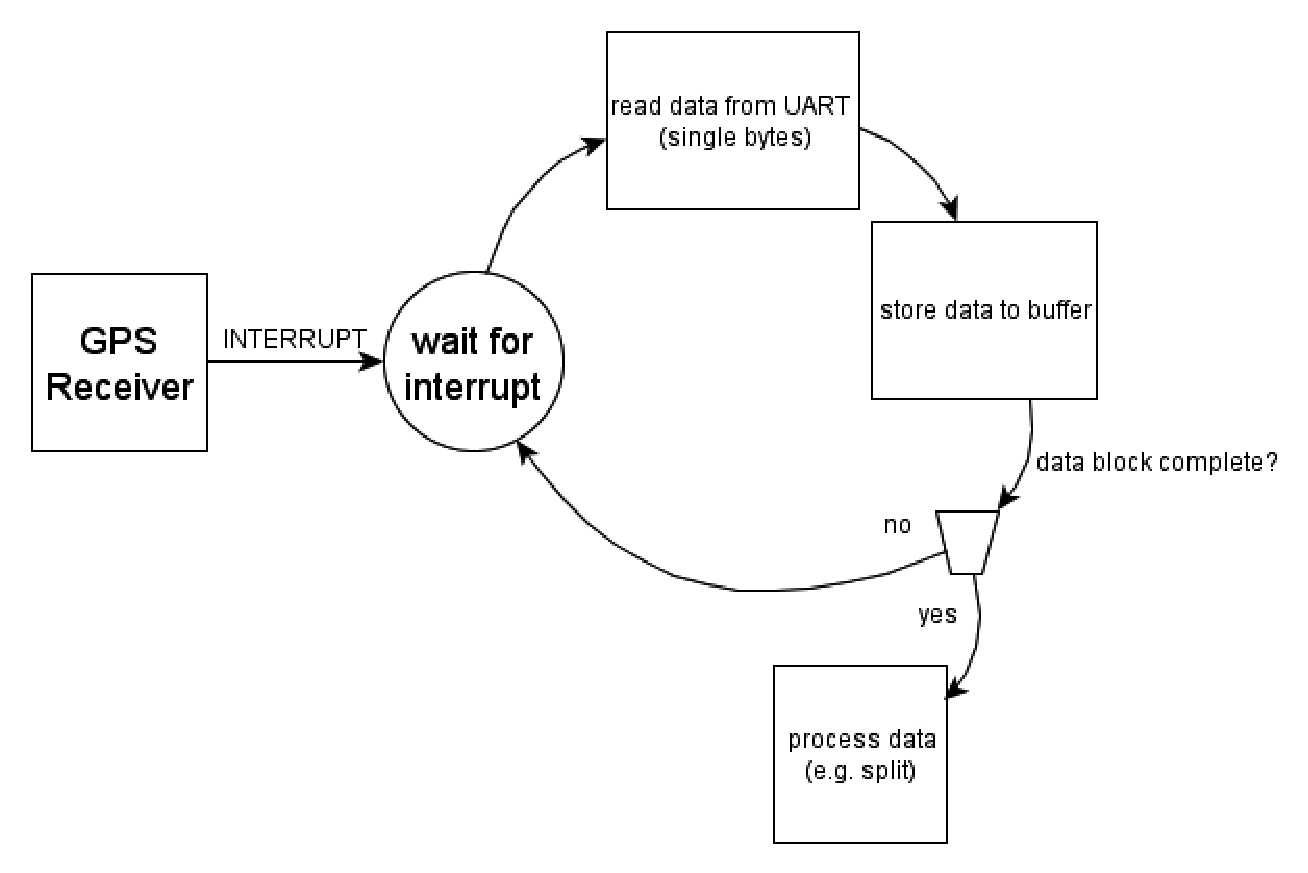
\includegraphics[width=\textwidth]{interrupt_function}
\end{figure}
\end{frame}

\begin{frame}
\frametitle{The graphic display}
\begin{columns}
        \column{.55\textwidth}
				\begin{figure}[th]
                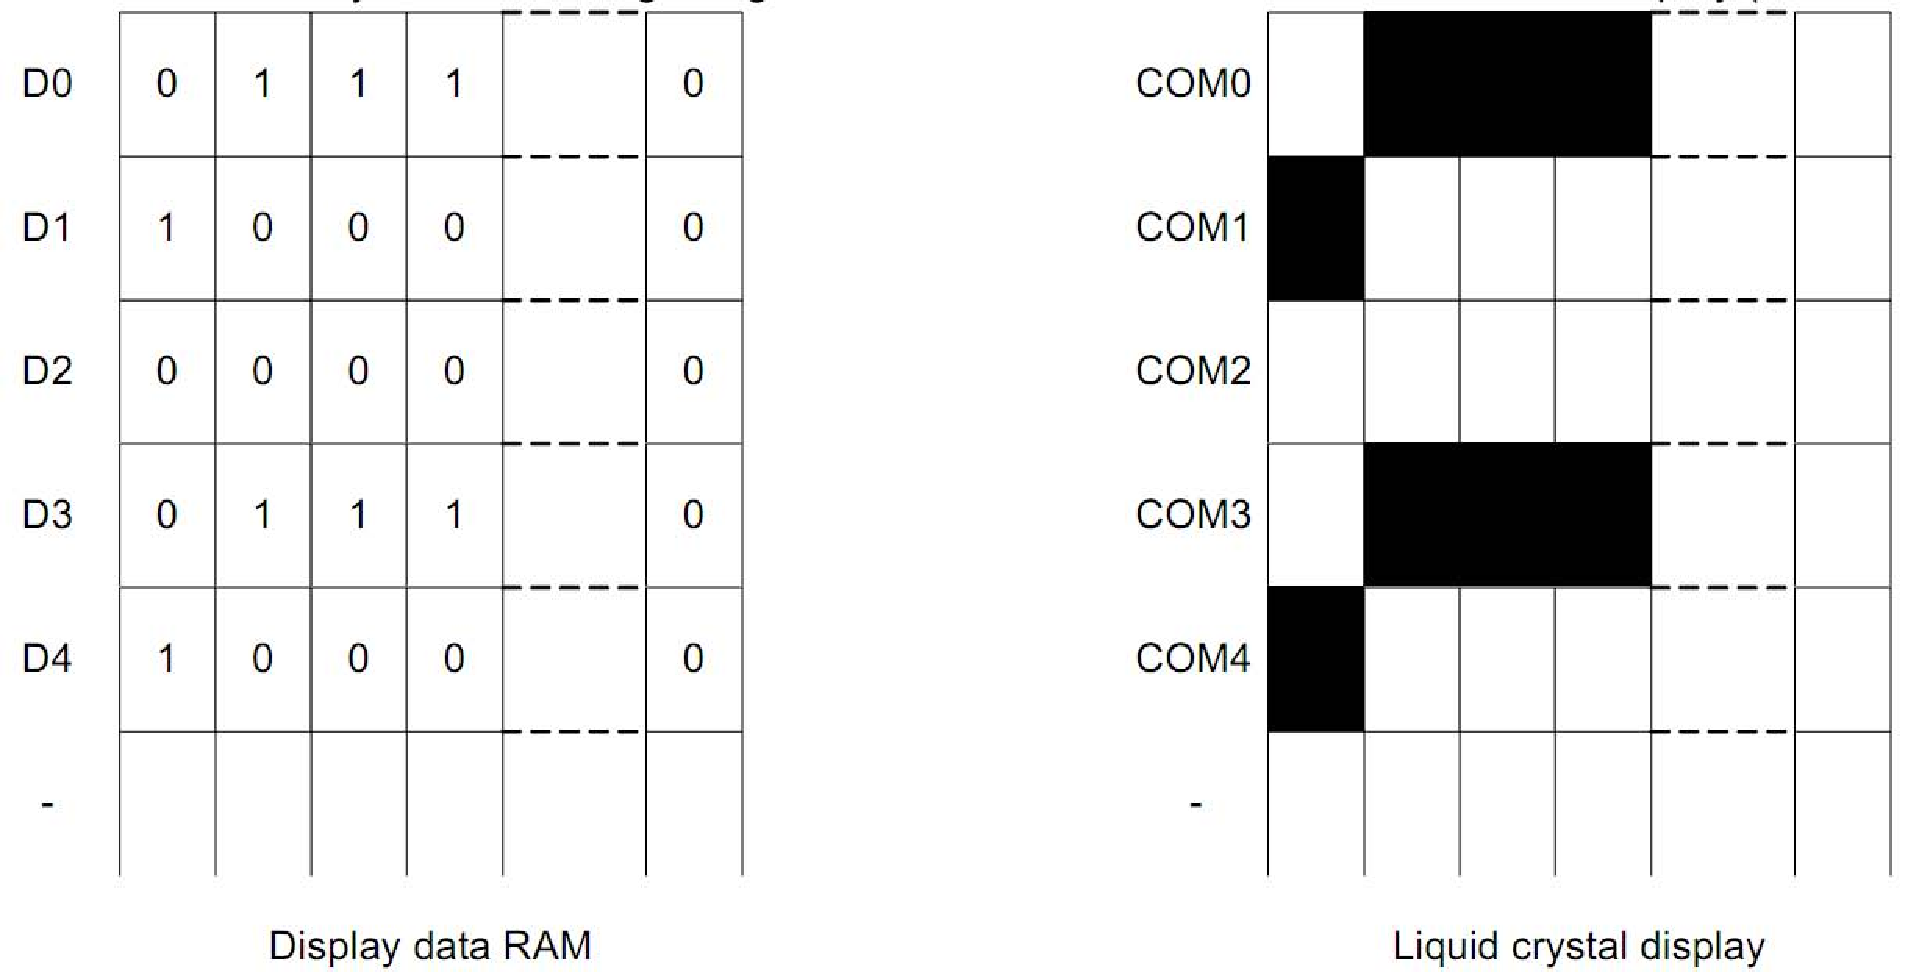
\includegraphics[width=\textwidth]{display_ram}
                \end{figure}
        \column{.45\textwidth}
                \begin{itemize}
                \item internal RAM organized in pages
                \item each page contains 8 rows and 128 columns
                \item software solution: linear storage within an array
                \end{itemize}
\end{columns}
\end{frame}

\begin{frame}
\frametitle{Display - Setting a single pixel}
\begin{itemize}
\item direct pixel access via display data RAM
\item virtual data representation is realized in linear order
\item setting a pixel with coordinates X and Y: $\textbf{INDEX} = (Y * 8) + (X / 8)$
\end{itemize}
\lstinputlisting[language=C,label=display_putpixel,caption=Setting a single pixel]{display_putpixel.c}
\end{frame}

\begin{frame}
\frametitle{GPS - Data storage}
\lstinputlisting[language=C,label=gps_data_buffer,caption=GPS data storage]{gps_data_buffer.c}
\end{frame}

\begin{frame}
\frametitle{Problems}
\begin{itemize}
\item ATmega32A RAM (2kB RAM too small)
\item Windows line endings (\textbackslash r\textbackslash n) in NMEA format
\item No provided SVN repository (used: Sourceforge)
\item No provided bug/feature tracker
\end{itemize}
\end{frame}

\section{Conclusion}
\subsection{Conclusion}
\begin{frame}
\frametitle{Project topics}
\begin{itemize}
\item missing project environment
\item very good support by Mr. Lenkowski
\item underestimated effort for planned features (even by the Professor)
\end{itemize}
\end{frame}

\begin{frame}
\frametitle{Ideas for future development}
Hardware:
\begin{itemize}
\item dimmable backlight via PWM
\item turning GPS receiver on/off via Mosfet
\item one board instead of our 4 layer solution
\item lipo batteries (flat)
\end{itemize}
\end{frame}

\begin{frame}
\frametitle{Ideas for future development}
Software:
\begin{itemize}
\item Integration of an OS (e.g. $\mu$ OS)
\item Implementation of further touch screen interaction applications
\item Rework to a 3-layer-architecture (Driver - Driver-Interfaces - Application)
\item Navigation features (e.g. Waypoints, Statistics,...)
\item PC application for communication via RS232
\item automated generated API documentation (Doxygen)
\end{itemize}
\end{frame}

\begin{frame}
\frametitle{Hardware receiving data...}
\begin{figure}
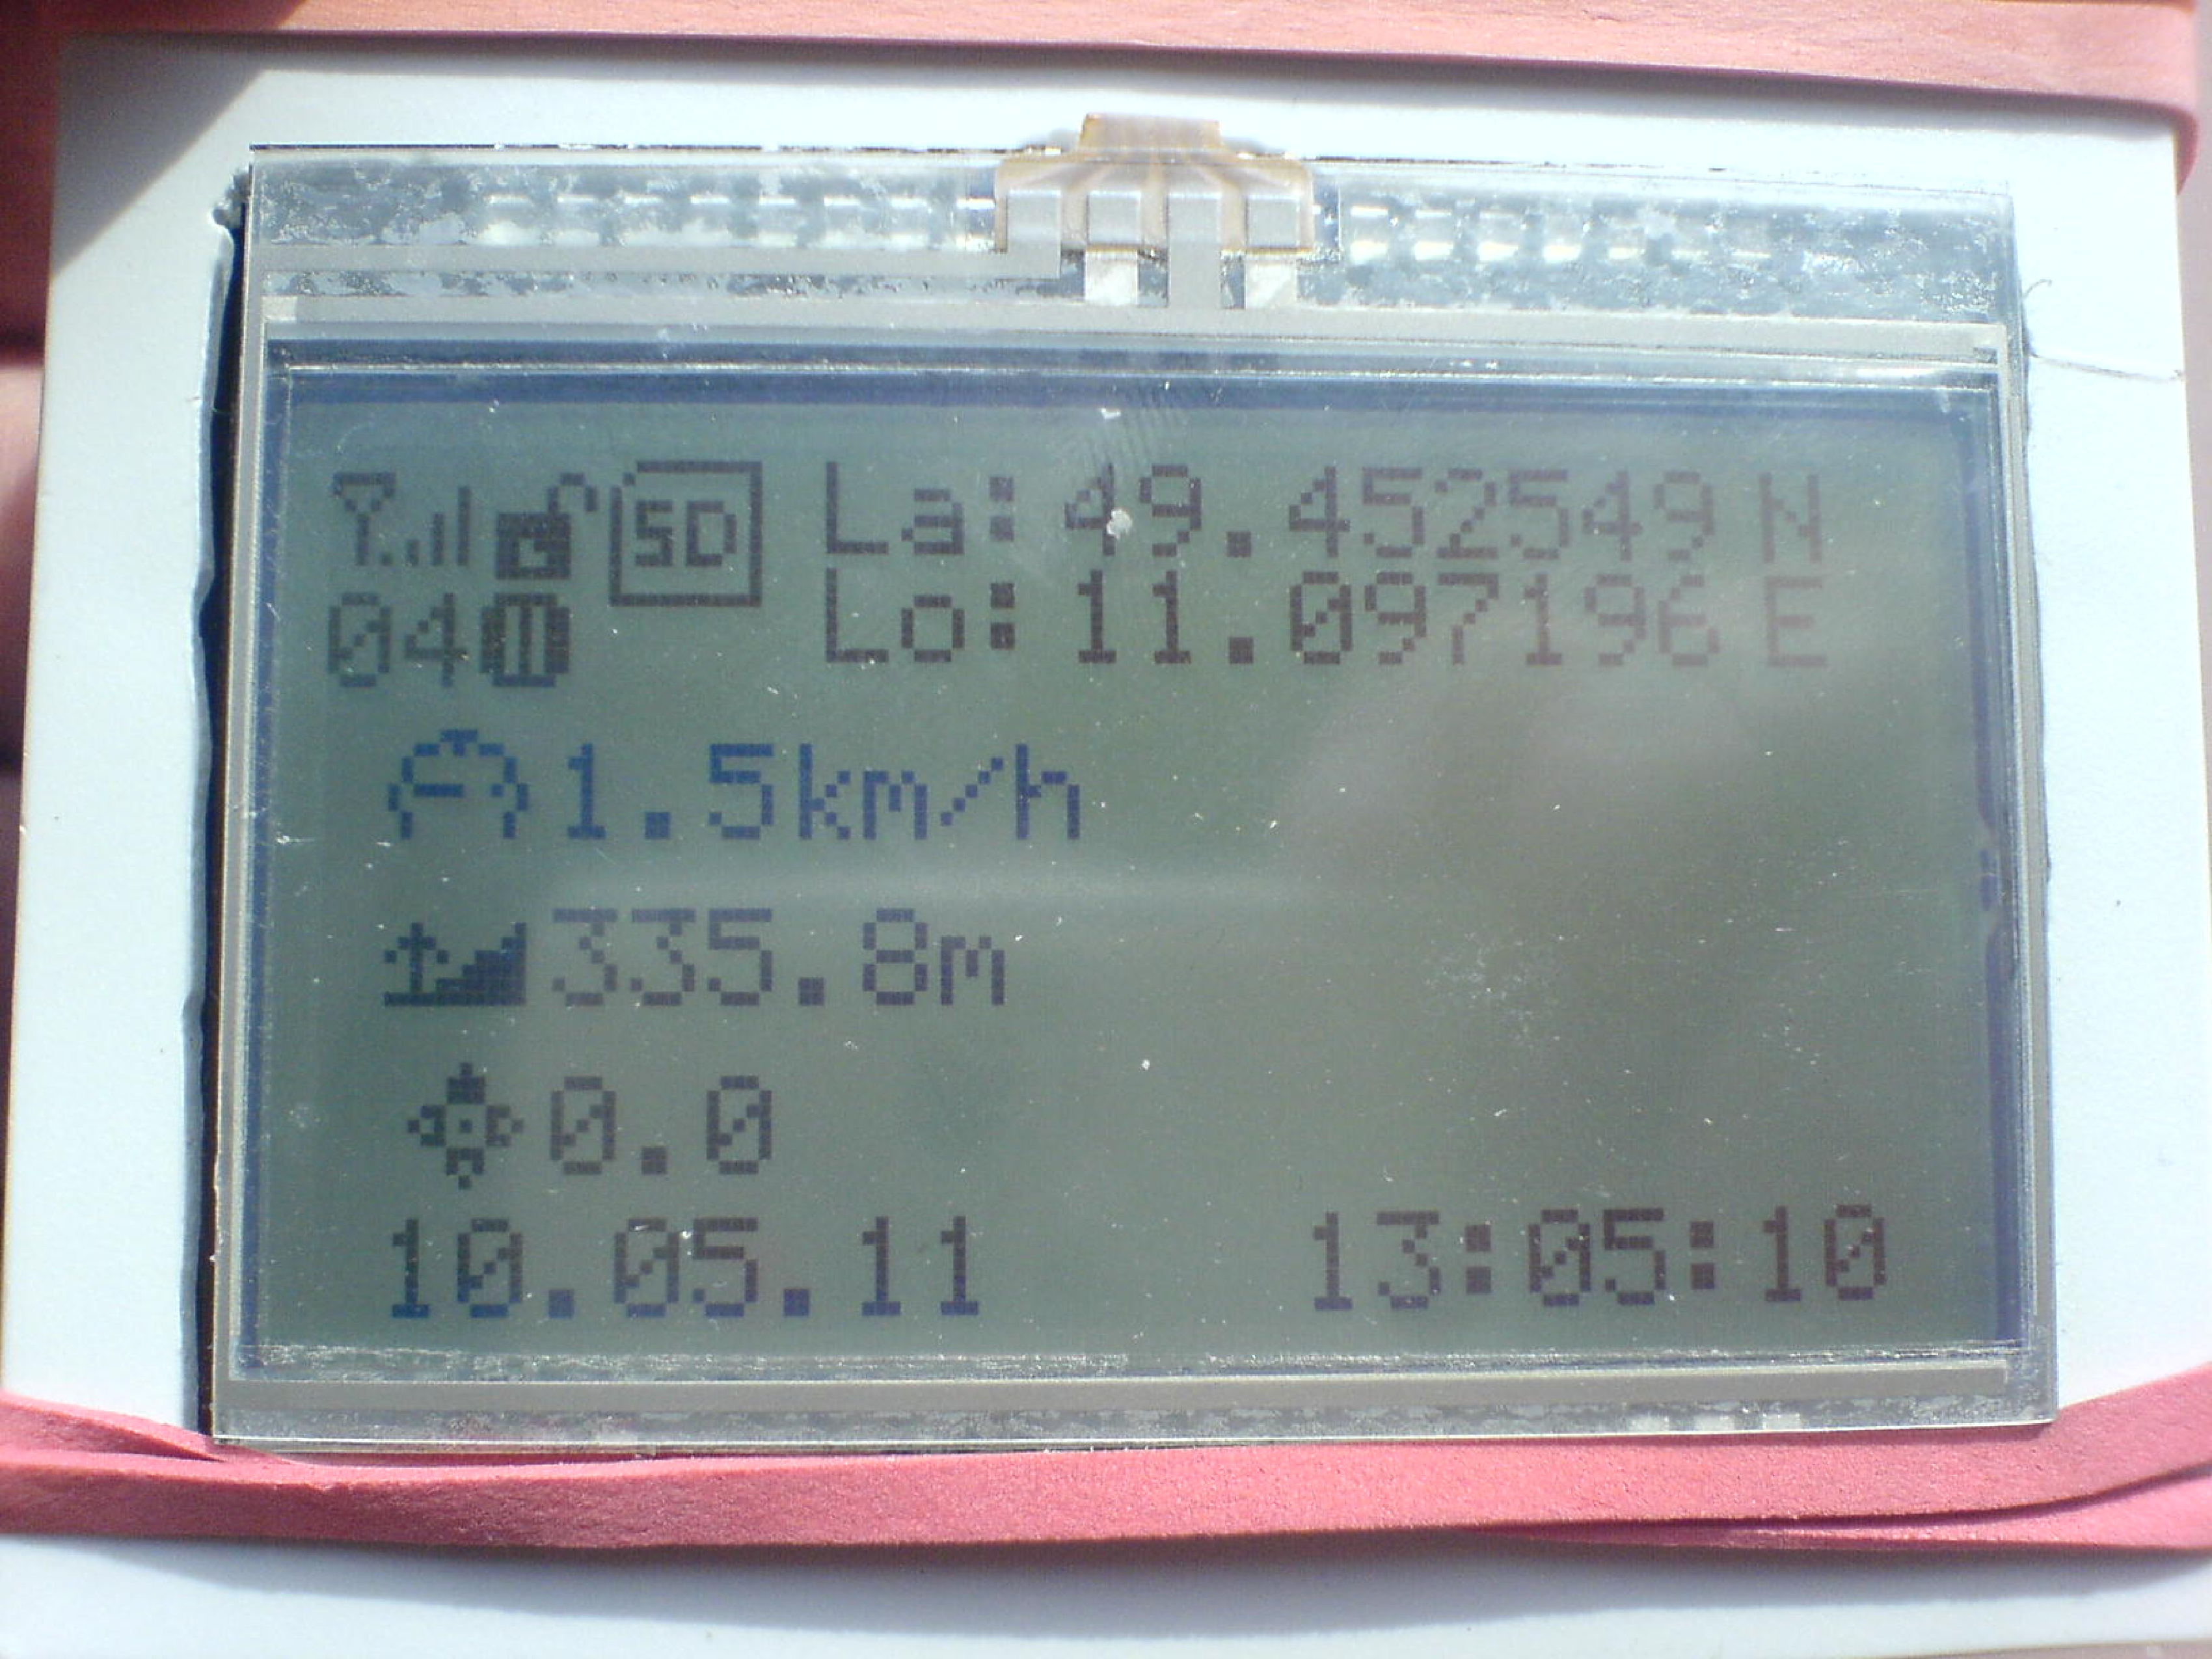
\includegraphics[width=\textwidth]{hardware_betrieb}
\end{figure}
\end{frame}

\begin{frame}
\frametitle{Reference}
\begin{itemize}
\item http://www.lcd-module.de/pdf/grafik/dogl128-6.pdf, Electronic Assembly
\item NL\_u-blox5\_Referenzmanual\_06102008\_571.pdf, u-blox 5 NMEA, UBX Protocol Specification
\item http://www.atmel.com/dyn/resources/prod\_documents/doc2593.pdf, ATmega644L datasheet
\end{itemize}
\end{frame}
\end{document}
